

%\part{Métodos de clasificación automática.}
%\frame{\partpage}

\chapter{Métodos de clasificación automática}

\section{Introducción}
\begin{frame}
\frametitle{Descripción del problema}
\begin{itemize}
\item<2->{Tenemos un conjunto de individuos con unas ciertas medidas multidimensionales.}
\item<3->{Queremos ver si existe una "forma natural" de clasificar a dichos individuos en grupos.}
\item<4->{Los grupos que formemos tienen que ser lo más homogéneos posible y las diferencias entre los grupos, lo más acentuadas posible.}
\end{itemize}
\end{frame}

\section{Algoritmo de las $k$-medias}
\begin{frame}
\frametitle{Introducción al algoritmo de las $k$-medias}
\begin{itemize}
\item<2->{En todo método de partición, partimos de $n$ individuos de los que se han tomado $p$ mediciones. O sea, tenemos una matriz $n\times p$ de $n$ individuos con $p$ variables:
$\vect{X}=
\begin{pmatrix}
x_{11}&x_{12}&\ldots&x_{1p} \\ 
x_{21}&x_{22}&\ldots&x_{2p} \\
\vdots&\vdots&\vdots&\vdots \\
x_{n1}&x_{n2}&\ldots&x_{no}
\end{pmatrix}$}
\item<3->{El objetivo del algoritmo de las $k$-medias es dividir los $n$ individuos en un número de conjuntos o grupos prefijado~$G$.}
\end{itemize}
\end{frame}

\section{Algoritmo de las $k$-medias}
\begin{frame}
\frametitle{Etapas del algoritmo de las $k$-medias}
\begin{itemize}
\item<2->{Se seleccionan $G$ puntos como centros de los puntos iniciales. Hay distintas formas de realizar dicha selección:
\begin{itemize}
\item asignando aleatoriamente los objetos a los grupos y tomando los centros de los grupos formados,
\item tomando como centros los $G$ más alejados entre sí,
\item seleccionando los centros ``a priori".
\end{itemize}}
\item<3->{Calcular las distancias euclídeas de cada elemento a los centros de los $G$ grupos, y asignar cada elemento al grupo de cuyo centro esté más próximo. La asignación se realiza secuencialmente y al introducir un nuevo elemento en un grupo se recalculan las coordenadas del nuevo centro del grupo.}
\item<4->{Definir un criterio de optimalidad y comprobar si reasignando alguno de los elementos mejora el criterio.}
\item<5->{Si no es posible mejorar el criterio de optimalidad, terminar el proceso.}
\end{itemize}
\end{frame}
\begin{frame}
\frametitle{Criterio de optimalidad.}
\begin{itemize}
\item<2->{Sea $x_{ijg}$ la medida $j$-ésima del individuo $i$-ésimo que pertenece al grupo~$g$. Definimos la suma de cuadrados dentro de los grupos $SCDG$ como:
$$
SCDG = \sum_{g=1}^G\sum_{j=1}^p\sum_{i=1}^{n_g} (x_{ijg}-\overline{x}_{jg})^2,
$$
donde $\overline{x}_{jg}$ es la media de esta variable en el grupo~$g$ y $n_g$ representa el número de elementos de grupo~$g$.}
\item<3->{Nuestro objetivo será encontrar aquella partición que minimice $SCDG$.}
\item<4->{La suma de cuadrados $SCDG$ puede escribirse como:
$$
SCDG = \sum_{g=1}^G\sum_{j=1}^{p}  n_g s_{jg}^2,
$$
donde $s_{jg}^2$ es la varianza de la variable $j$ en el grupo~$g$.}
\end{itemize}
\end{frame}

\begin{frame}
\frametitle{Criterio de optimalidad.}
\begin{itemize}
\item<2->{Escribamos matricialmente el criterio de optimalidad:
$$
SCDG = \sum_{g=1}^G\sum_{i=1}^{n_g} (\vect{x}_{ig}-\overline{\vect{x}}_g)^\top (\vect{x}_{ig}-\overline{\vect{x}}_g),
$$
donde $\vect{x}_{ig}$ sería el vector de los $j$ valores del individuo $i$-ésimo dentro del grupo~$g$ y $\overline{\vect{x}}_g$ sería el vector de medias de los $g$ grupos.}
\item<3->{El valor anterior de dentro del sumatorio es la distancia euclídea entre el individuo $i$-ésimo dentro del grupo $g$ y la media dentro del grupo~$g$. Si nombramos $d^2(i,g)$ a dicha distancia, podemos escribir: $$SCDG=\sum_{g=1}^G\sum_{i=1}^{n_g} d^2(i,g).$$}
\end{itemize}
\end{frame}
\begin{frame}
\frametitle{Criterio de optimalidad.}
\begin{itemize}
\item<2->{Usando que $ (\vect{x}_{ig}-\overline{\vect{x}}_g)^\top (\vect{x}_{ig}-\overline{\vect{x}}_g) =tr( (\vect{x}_{ig}-\overline{\vect{x}}_g) (\vect{x}_{ig}-\overline{\vect{x}}_g))^\top$ (ejercicio), podemos escribir la suma de cuadrados como:
$$
SCDG=tr\left( \sum_{g=1}^G\sum_{i=1}^{n_g} (\vect{x}_{ig}-\overline{\vect{x}}_g) (\vect{x}_{ig}-\overline{\vect{x}}_g))^\top \right),
$$
donde $tr$ significa traza.}
\item<3->{Nombrando $\vect{W}$ a la matriz $ \sum_{g=1}^G\sum_{i=1}^{n_g} (\vect{x}_{ig}-\overline{\vect{x}}_g) (\vect{x}_{ig}-\overline{\vect{x}}_g))^\top$, tenemos que el criterio de optimalidad equivale a minimizar la traza de la matriz~$\vect{W}$.}
\end{itemize}
\end{frame}

\begin{frame}
\frametitle{Ejemplo}
\begin{itemize}
\item<2->{La siguiente tabla muestra el gasto medio en varios tipos de comida para distintos tipos de familias en Francia: trabajadores manuales (TM), empleados (EM) y directivos (DIR) con distintos número de hijos: 2, 3, 4 o 5 hijos.

Significado de las siglas:
\begin{description}
\item[TF] Tipo familia
\item[P] Pan
\item[VE] Vegetales
\item[F] Fruta
\item[C] Carne
\item[A] Aves
\item[L] Leche
\item[VI] Vino
\end{description}
}
\end{itemize}
\end{frame}
\begin{frame}
\frametitle{Ejemplo}
\begin{itemize}
\item<2->{\begin{tabular}{|r|r|r|r|r|r|r|r|}
\hline
TF&P&VE&F&C&A&L&VI\\\hline
TM2&332&428&354&1437&526&247&427\\\hline
EM2&293&559&388&1527&567&239&258\\\hline
DIR2&372&767&562&1948&927&235&433\\\hline
TM3&406&563&341&1507&544&324&407\\\hline
EM3&386&608&396&1501&558&319&363\\\hline
DIR3&438&843&689&2345&1148&243&341\\\hline
TM4&534&660&367&1620&638&414&407\\\hline
EM4&460&699&484&1856&762&400&416\\\hline
DIR4&385&789&621&2366&1149&304&282\\\hline
TM5&655&776&423&1848&759&495&486\\\hline
EM5&584&995&548&2056&893&518&319\\\hline
DIR5&515&1097&887&2630&1167&561&284\\\hline
\end{tabular}}
\end{itemize}
\end{frame}
\begin{frame}
\frametitle{Ejemplo}
\begin{itemize}
\item<2->{Elegiremos $G=3$. Elegiremos como centros de los valores iniciales las medias de los $4$ primeros individuos, luego las medias de los individuos $5$ al $8$ y por último las medias de los individuos $9$ al $12$. O sea, elegimos como grupos iniciales los siguientes:
Grupo 1: individuos $1$, $2$, $3$ y $4$. Grupo 2: individuos $5$, $6$, $7$ y $8$ y Grupo 3: individuos $9$, $10$, $11$ y $12$. Las coordenadas de los $3$ centros iniciales son las siguientes:
$$
{\small \begin{pmatrix}
350.75 & 579.25 & 411.25 & 1604.75 & 641.0 & 261.25 & 381.25 \\
454.50 & 702.50 & 484.00 & 1830.50 & 776.5 & 344.00 & 381.75 \\
534.75 & 914.25 & 619.75 & 2225.00 & 992.0 & 469.50 & 342.75 \\
\end{pmatrix}}
$$}
\end{itemize}
\end{frame}
\begin{frame}
\frametitle{Ejemplo}
\begin{itemize}
\item<2->{En el gráfico siguiente observamos la proyección de las dos primeras variables de los individuos junto con los centros de los grupos iniciales (en rojo):
\vskip0.25cm
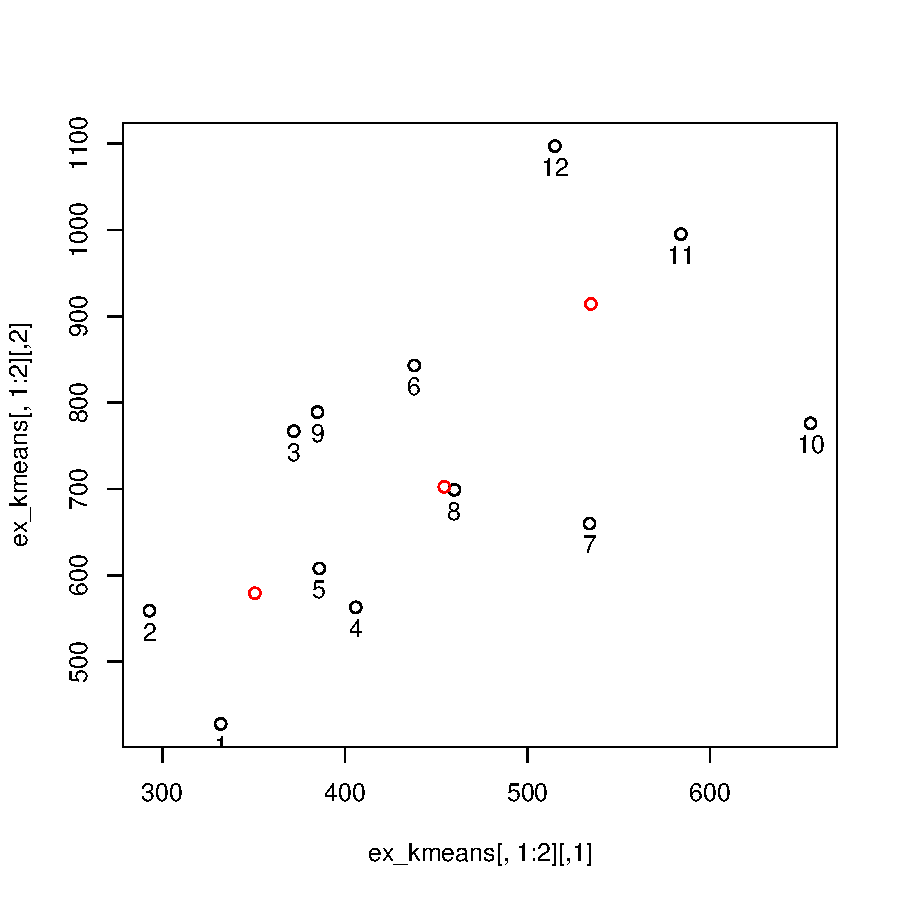
\includegraphics[scale=0.4]{kmeans1.pdf}}
\end{itemize}
\end{frame}
\begin{frame}
\frametitle{Ejemplo}
\begin{itemize}
\item<-2>{Vamos a aplicar el algoritmo de k-means a nuestro ejemplo. El valor inicial de $SCDG$ es $1916875$. Calculemos primero el grupo más cercano de cada individuo hallando la distancia entre éste y el centro correspondiente:
\begin{itemize}
\item Individuo 1: distancias de $(332,428,354,1437,526,247,427)$ a cada uno de los centros: 
$$
{\tiny
\begin{array}{rl}
d((332,428,\ldots ,427), (350.75, 579.25 ,\ldots , 381.25)) = & 264.895, \\
d((332,428,\ldots ,427), (454.50, 702.50 , \ldots , 381.75 ) = & 579.945, \\
d((332,428,\ldots ,427), (534.75, 914.25, \ldots , 342.75 ) = & 1114.883.
\end{array}}$$
Por tanto, el grupo correspondiente al primer individuo es el primero. No hay ningún cambio.
\item Con el individuo 2, tampoco hay cambios. En cambio con el individuo 3, resulta que el grupo más cercano es el grupo~2. Por tanto, cambiamos los grupos por: 
$$
G1 = \{ 1,2,4\},\ G2 = \{3,5,6,7,8\},\ G3 = \{ 9,10,11,12\}.
$$
\end{itemize}
}
\end{itemize}
\end{frame}

\begin{frame}
\frametitle{Ejemplo}
\begin{itemize}
\item<2->{El nuevo valor de $SCDG$ es $1622739$. Ha habido por tanto una mejora. Los nuevos centros son:
$$
{\tiny \begin{pmatrix}
343.667 & 516.667 & 361.000 &  1490.333 &  545.667 & 270.000 &  364.000 \\
438.000 & 715.400 &  499.600 & 1854.000 &  806.600 &  322.200 &  392.000  \\
534.750 & 914.250 &  619.750 &  2225.000 &  992.000 & 469.500 &  342.750 \\
\end{pmatrix}}
$$}
\item<3->{Volvemos a mirar el grupo más cercano de cada individuo: individuo 1: grupo 1 (no hay cambios); individuo 2: grupo 1 (no hay cambios); individuo 3: grupo 2 (no hay cambios); individuo 4:  grupo 1 (no hay cambios); individuo 5: grupo 1. Por tanto, cambiamos los grupos por: 
$$
G1 = \{ 1,2,4,5\},\ G2 = \{3,6,7,8\},\ G3 = \{ 9,10,11,12\}.
$$
El nuevo valor de $SCDG$ es $1367967$. Se sigue mejorando. Los nuevos centros son:
$$
{\tiny \begin{pmatrix}
354.250 &  539.500 &  369.750 &  1493.000 &  548.750 &  282.250 &  363.750 \\
451.000 &  742.250 &  525.500 &  1942.250 &  868.750 &  323.000 &  399.250 \\
534.75 & 914.250 &  619.750 &  2225.000 &  992.000 &  469.500 & 342.750 \\
\end{pmatrix}}
$$}
\end{itemize}
\end{frame}

\begin{frame}
\frametitle{Ejemplo}
\begin{itemize}
\item<2->{La tabla siguiente va mostrando los pasos del algoritmo donde la primera columna nos indica el individuo que va cambiando de grupo:
\begin{center}
{\tiny\begin{tabular}{|c|c|c|c|l|}\hline
&Grupo 1& Grupo 2& Grupo 3&$SCDG$\\\hline
$6$&$\{1,2,4,5\}$&$\{3,7,8\}$&$\{6,9,10,11,12\}$&$1072675$\\\hline
$10$&$\{1,2,4,5\}$&$\{3,7,8,10\}$&$\{6,9,11,12\}$&$709037.8$\\\hline
$11$&$\{1,2,4,5\}$&$\{3,7,8,10,11\}$&$\{6,9,12\}$&$632336.1$\\\hline
$7$&$\{1,2,4,5,7\}$&$\{3,8,10,11\}$&$\{6,9,12\}$&$564800.9$\\\hline
\end{tabular}}
\end{center}}
\end{itemize}
\end{frame}
\subsection{Propiedades del algoritmo de $k$-means}
\begin{frame}
\frametitle{Propiedades del algoritmo de $k$-means}
\begin{itemize}
\item<2->{El algoritmo no es invariante ante cambios de escala. Por tanto, si las variables van en unidades distintas, conviene estandarizarlas antes de aplicar el algoritmo.}
\item<3->{El algoritmo produce grupos aproximadamente esféricos ya que tiende a minimizar las distancias euclídeas entre los puntos y sus medias de grupo.}
\end{itemize}
\end{frame}

\subsection{Elección del número de grupos}
\begin{frame}
\frametitle{Elección del número de grupos}
\begin{itemize}
\item<2->{El procedimiento habitual de elegir cuántos grupos hay que usar en el algoritmo de $k$-means es el llamado test $F$ de reducción de variabilidad.}
\item<3->{Dicho test consiste en calcular:
$$
F=\frac{SCDG(G)-SCDG(G+1)}{SCDG(G+1)/(n-G-1)},
$$
donde se compara la variabilidad al aumentar un grupo con la varianza promedio. El valor obtenido se compara con el valor crítico de una distribución $F$ de $p$ y $p(n-G-1)$ grados de libertad. Hay que decir que dicha regla no está muy justificada ya que los datos no tienen porqué verificar las hipótesis necesarias para aplicar la distribución~$F$.}
\end{itemize}
\end{frame}
\begin{frame}
\frametitle{Ejemplo}
\begin{itemize}
\item<2->{En la tabla siguiente observamos los valores de $SCDG$ para distintas elecciones de $G$:
\begin{center}
\begin{tabular}{|c|c|c|}\hline
$G$&$SCDG$&$F$\\\hline
$3$&$564800.9$& \\\hline
$4$&$363066.1$&$\frac{(564800.9-363066.1)}{363066.1/(12-3-1)}=4.44$\\\hline
$5$&$255134.8$&$\frac{(363066.1-255134.8)}{255134.8/(12-4-1)}=2.96$\\\hline
$6$&$153977.9$&$\frac{(255134.8-153977.9)}{153977.9/(12-5-1)}=3.94$\\\hline
$7$&$109217.7$&$\frac{153977.9-109217.7}{109217.7/(12-6-1)}=2.05$\\\hline
\end{tabular}
\end{center}}
\item<3->{La reducción de la variabilidad más acentuada se produce al pasar de $3$ a $4$ grupos. Si hallamos el valor crítico (para $\alpha =0.05$) de la distribución $F$ con $p=7$ y $p(n-G-1)=7\cdot (12-3-1)=56$ grados de libertad, obtenemos $F_{0.95,7,56}=2.18$. Como $4.44 > 2.18$, concluimos que la variabilidad se ha reducido y, según este criterio, escogeríamos $G=4$ como el número de grupos óptimo.}
\end{itemize}
\end{frame}
\section{Métodos jerárquicos}

\begin{frame}
\frametitle{Introducción}
\begin{itemize}
\item<2->{Los métodos jerárquicos parten de una matriz de distancias o similaridades. O sea, suponemos que tenemos una matriz $D$ $n\times n$ que nos dice la distancia entre los individuos o elementos de la muestra: $d_{ij}:$ distancia entre el individuo~$i$ y el individuo~$j$. }
\item<3->{A partir de la matriz de distancias, se define el algoritmo de construcción de grupos. O sea, usando la matriz de distancias definida anteriormente, indicar cómo se formarán los distintos grupos.}
\end{itemize}
\end{frame}
\subsection{Matriz de distancias}
\begin{frame}
\frametitle{Cómo calcular la matriz de distancias}
\begin{itemize}
\item<2->{Recordemos que tenemos $n$ individuos de los que se han tomado $p$ mediciones:
$\vect{X}=
\begin{pmatrix}
x_{11}&x_{12}&\ldots&x_{1p} \\ 
x_{21}&x_{22}&\ldots&x_{2p} \\
\vdots&\vdots&\vdots&\vdots \\
x_{n1}&x_{n2}&\ldots&x_{np}
\end{pmatrix}$}
\item<3->{A partir de la matriz $\vect{X}$ hemos de construir una matriz de similaridad-disimilaridad $\vect{D}$ $n\times n$ entre los objetos:
$\vect{D}=
\begin{pmatrix}
d_{11}&d_{12}&\ldots&d_{1n} \\ 
d_{21}&d_{22}&\ldots&d_{2p} \\
\vdots&\vdots&\vdots&\vdots \\
d_{n1}&d_{n2}&\ldots&d_{nn}
\end{pmatrix}$}
\item<4->{En el  caso en que $\vect{D}$ sea una matriz de similaridad, cuánto menor sean los valores $d_{ij}$, más alejados estarán los individuos $i$ y $j$ y en el segundo caso, más cercanos estarán.}
\end{itemize}
\end{frame}
\subsection{Datos binarios}
\begin{frame}
\frametitle{Introducción}
\begin{itemize}
\item<2->{Supongamos que la matriz $\vect{X}$ sólo coge los valores $0$ o $1$. En este caso, diremos que la estructura de los datos es binaria.}
\item<3->{De cara a definir la matriz de similaridad, consideremos los datos referentes al individuo~$i$ (columna $i$ de la matriz $\vect{X}$: $(x_{i1},\ldots,x_{ip})^\top$) y al individuo~$j$ (columna $j$ de la matriz $\vect{X}$: $(x_{j1},\ldots,x_{jp})^\top$)}
\item<4->{Definimos las cantidades siguientes:
$$
\begin{array}{rl}
a_1 = & \sum_{k=1}^p \mathcal{I}(x_{ik}=x_{jk}=1), \\
a_2 = & \sum_{k=1}^p \mathcal{I}(x_{ik}=0, x_{jk}=1), \\
a_3 = & \sum_{k=1}^p \mathcal{I}(x_{ik}=1, x_{jk}=0), \\
a_4 = & \sum_{k=1}^p \mathcal{I}(x_{ik}=x_{jk}=0),
\end{array}
$$
donde $\mathcal{I}(\mbox{condición})$ cuenta cuantos elementos de la matriz $\vect{X}$ cumplen la condición.}
\end{itemize}
\end{frame}
\begin{frame}
\frametitle{Definición de la matriz de distancias}
\begin{itemize}
\item<2->{Definimos la similaridad entre los individuos $i$ y $j$ como:
$$
d_{ij}=\frac{a_1 + \delta a_4}{a_1 + \delta a_4 +\lambda (a_2 + a_3)}.
$$
}
\item<3->{Los parámetros $\delta$ y $\lambda$ son factores de peso. La tabla siguiente muestra ejemplos de similaridades más comunes:
\vskip 0.25cm
\begin{tabular}{|l|r|r|c|}
\hline
Nombre&$\delta$&$\lambda$&Definición\\\hline
Jaccard&$0$&$1$&$\frac{a_1}{a_1 + a_2 +a_3}$ \\\hline
Tanimoto&$1$&$2$&$\frac{a_1+a_4}{a_1+2(a_2+a_3)+a_4}$\\\hline
Simple&$1$&$1$&$\frac{a_1 + a_4}{p}$\\\hline
Rusell y Rao&-&-&$\frac{a_1}{p}$\\\hline
Dice&$0$&$0.5$&$\frac{2a_1}{2a_1 + a_2 +a_3}$ \\\hline
Kulczynski&-&-&$\frac{a_1}{a_2 + a_3}$\\\hline
\end{tabular}}
\end{itemize}
\end{frame}
\begin{frame}
\frametitle{¿Por qué no se usa la distancia euclídea?}
\begin{itemize}
\item<2->{La distancia euclídea no sería adecuada en este caso ya que trata los valores $0$ y $1$ de la misma forma y en la mayoría de aplicaciones donde se tratan datos binarios, deben ser tratados de formas distintas.}
\item<3->{Por ejemplo, si $x_{ik}=1$ significa que el individuo $i$ tiene un cierto conocimiento sobre el lenguaje~$k$ y si $x_{ik}=0$ significa que no lo tiene, el valor $x_{ik}=0$ tiene que tratarse de forma distinta del valor $x_{ik}=1$.}
\end{itemize}
\end{frame}
\begin{frame}
\frametitle{Ejemplo}
\begin{itemize}
\item<2->{Consideremos $3$ tipos de marca de automóviles, Renault, Rover y Toyota. Se ha realizado una encuesta en $40$ personas para que opinen de las variables siguientes: Economía (EC), servicio (SER), valor no depreciado (V), precio (P)(valor $1$ para los coches más baratos), diseño (DI), deportividad (DE), seguridad (SEG) y facilidad de Manejo (FM). Los resultados van de $1$ (muy bueno) a $6$ (muy malo).}
\item<3->{Las medias de las valoraciones de los $40$ encuestados son:
\vskip 0.25cm
\begin{tabular}{|l|c|c|c|c|c|c|c|c|}
\hline
Modelo&EC&SER&V&P&DI&DE&SEG&FM\\\hline
Renault&2.7&3.3&3.4&3.0&3.1&3.4&3.0&2.7\\\hline
Rover&3.9&2.8&2.6&4.0&2.6&3.0&3.2&3.0\\\hline
Toyota&2.5&2.9&3.4&3.0&3.2&3.1&3.2&2.8\\\hline
\end{tabular}
}
\end{itemize}
\end{frame}
\begin{frame}
\frametitle{Ejemplo}
\begin{itemize}
\item<2->{Sea $\vect{X}$ la matriz de datos anterior:
$$
\vect{X}=
\begin{pmatrix}
2.7&3.3&3.4&3.0&3.1&3.4&3.0&2.7\\
3.9&2.8&2.6&4.0&2.6&3.0&3.2&3.0\\
2.5&2.9&3.4&3.0&3.2&3.1&3.2&2.8
\end{pmatrix}
$$
Se trata de una matriz $3\times 8$ de $3$ individuos con $8$ variables.}
\item<3->{A partir de la matriz anterior, construimos la matriz binaria siguiente:
$y_{ik}=\left\{\begin{array}{ll}
1,&\mbox{si } x_{ik}> \overline{x}_k, \\
0,&\mbox{en caso contrario.}
\end{array}
\right.$}
\item<4->{La matriz $\vect{Y}$ es:
$$
\vect{Y}=
\begin{pmatrix}
 0  &  1  &  1 &   0  &  1  &  1  &  0  &   0  \\
  1  &   0  &   0  &   1  &   0  &   0 &    1 &    1 \\
  0  &   0  &   1  &   0  &   1  &   0 &    1  &   0\\
\end{pmatrix}
$$
}
\end{itemize}
\end{frame}
\begin{frame}
\frametitle{Ejemplo}
\begin{itemize}
\item<2->{Si aplicamos la medida de Jaccard, obtenemos la matriz siguiente de similaridad:
$$
\vect{D}=
\begin{pmatrix}
1.000 & 0.000 & 0.400 \\
&1.000 & 0.167 \\
&&1.000
\end{pmatrix}
$$
}
\item<3->{La medida de Tanimoto da el siguiente resultado:
$$
\vect{D}=
\begin{pmatrix}
1.000 & 0.000 & 0.455 \\
&1.000 & 0.231 \\
&&1.000
\end{pmatrix}
$$}
\item<4->{La medida simple da como matriz de similaridad:
$$
\vect{D}=
\begin{pmatrix}
1.000 & 0.000 & 0.625 \\
&1.000 & 0.375 \\
&&1.000
\end{pmatrix}
$$}
\end{itemize}
\end{frame}
\subsection{Datos continuos}
\begin{frame}
\frametitle{Introducción}
\begin{itemize}
\item<2->{En el caso general de datos continuos, se usan las distancias generadas por las normas $L_r,\ r\geq 1$. Esto es, la distancia entre el individuo $i$ (fila $i$ de la matriz $\vect{X}$: $(x_{i1},\ldots,x_{ip})^\top$) y al individuo~$j$ (fila $j$ de la matriz $X$: $(x_{j1},\ldots,x_{jp})^\top$) viene dada por:
$$
d_{ij}=||\vect{x_i} - \vect{x_j}||_r = \left(\sum_{k=1}^p |x_{ik} - x_{jk}|^r\right)^{\frac{1}{r}}.
$$
}
\item<3->{Es claro que en este caso $d_{ii}=0$. Por tanto, usamos una matriz de distancias o disimilaridad. Si $r=2$, tenemos la distancia euclídea usual.}
\end{itemize}
\end{frame}
\begin{frame}
\frametitle{Escalado de los datos}
\begin{itemize}
\item<2->{Una suposición usual es que los datos estén en la misma escala. Si no fuese el caso, la definición de la matriz de distancias se realiza mediante una métrica $\vect{A}$. En el caso de la distancia euclídea, la modificación sería: 
$$
d_{ij}^2=||\vect{x_i} - \vect{x_j}||_\vect{A} = (\vect{x_i} - \vect{x_j})^\top \vect{A} (\vect{x_i} - \vect{x_j}).
$$}
\item<3->{La métrica $\vect{A}$ más usada es la siguiente: 
$$
\vect{A}= \mbox{diag} \left( s_{\vect{x_1}\vect{x_1}}^{-1},\ldots,s_{\vect{x_p}\vect{x_p}}^{-1}
\right),
$$
donde $s_{\vect{x_k}\vect{x_k}}$ es la varianza de la variable $k$-ésima.}
\item<4->{La distancia euclídea quedará de la forma siguiente:
$$
d_{ij}^2 = \sum_{k=1}^p \frac{\left(x_{ik}-x_{jk}\right)^2}{s_{\vect{x_k}\vect{x_k}}}.
$$}
\end{itemize}
\end{frame}
\begin{frame}
\frametitle{Ejemplo}
\begin{itemize}
\item<2->{Recordemos el ejemplo del gasto medio en varios tipos de comida para distintos tipos de familias en Francia: trabajadores manuales (TM), empleados (EM) y directivos (DIR) con distintos número de hijos: 2, 3, 4 o 5 hijos.

Significado de las siglas:
\begin{description}
\item[TF] Tipo familia
\item[P] Pan
\item[VE] Vegetales
\item[F] Fruta
\item[C] Carne
\item[A] Aves
\item[L] Leche
\item[VI] Vino
\end{description}
}
\end{itemize}
\end{frame}
\begin{frame}
\frametitle{Ejemplo}
\begin{itemize}
\item<2->{\begin{tabular}{|r|r|r|r|r|r|r|r|}
\hline
TF&P&VE&F&C&A&L&VI\\\hline
TM2&332&428&354&1437&526&247&427\\\hline
EM2&293&559&388&1527&567&239&258\\\hline
DIR2&372&767&562&1948&927&235&433\\\hline
TM3&406&563&341&1507&544&324&407\\\hline
EM3&386&608&396&1501&558&319&363\\\hline
DIR3&438&843&689&2345&1148&243&341\\\hline
TM4&534&660&367&1620&638&414&407\\\hline
EM4&460&699&484&1856&762&400&416\\\hline
DIR4&385&789&621&2366&1149&304&282\\\hline
TM5&655&776&423&1848&759&495&486\\\hline
EM5&584&995&548&2056&893&518&319\\\hline
DIR5&515&1097&887&2630&1167&561&284\\\hline
\end{tabular}}
\end{itemize}
\end{frame}
\begin{frame}
\frametitle{Ejemplo}
\begin{itemize}
\item<2->{La matriz de distancia euclidea para los datos anteriores es:
%\vskip 0.25cm
%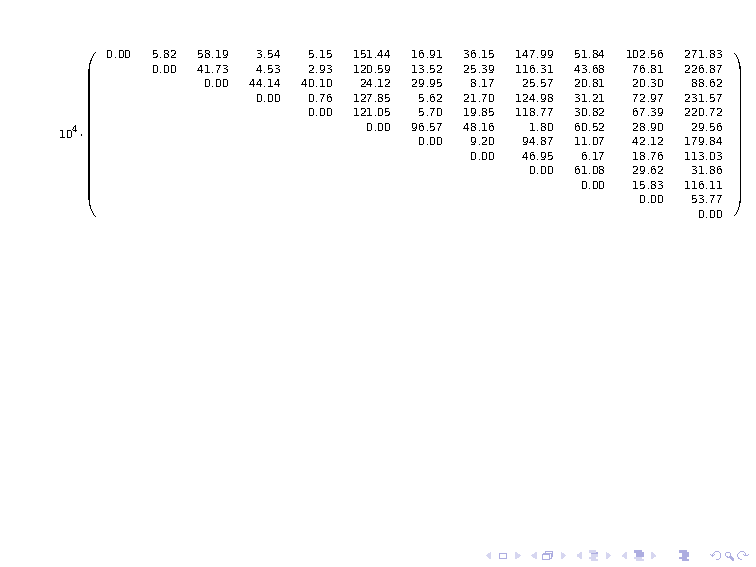
\includegraphics[scale=0.7]{dist_eucl.pdf}}
\begin{center}
{\tiny
\begin{tabular}{|@{}r@{}|@{}r@{}|@{}r@{}|@{}r@{}|@{}r@{}|@{}r@{}|@{}r@{}|@{}r@{}|@{}r@{}|@{}r@{}|@{}r@{}|@{}r@{}|}\hline
0.00 &&&&&&&&&&&\\\hline                                                                                                                         
241.34&    0.00&&&&&&&&&&\\        \hline                                                                                                        
762.82&  645.96 &    0.00&&&&&&&&&\\\hline                                                                                                     
188.21 &  212.95 &  664.36 &    0.00&&&&&&&&\\        \hline                                                                                  
226.89& 171.16&  633.21&   87.42&    0.00&&&&&&&\\         \hline                                                                      
1230.63&1098.12&  491.16& 1130.71& 1100.22 &    0.00&&&&&&\\         \hline                                                           
411.24&  367.75&  547.30&  237.01&  238.69&  982.71 &   0.00&&&&&\\              \hline                                           
601.26 &  503.84& 285.75&  465.88&  445.55&  694.00&  303.37&    0.00&&&&\\     \hline                                         
1216.50&1078.47&  505.67& 1117.97& 1089.81&  134.14&  974.02&  685.23&    0.00&&&\\      \hline                             
719.99&  660.90&  456.21&  558.64&  555.18&  777.94&  332.66&  248.34&  781.53&    0.00&&\\      \hline                  
1012.71&  876.39&  450.59&  854.25&  820.89&  537.55&  648.97&  433.11&  544.21&  397.83&    0.00&\\    \hline         
1648.73& 1506.22&  941.37& 1521.75& 1485.66&  543.70& 1341.05& 1063.15&  564.44& 1077.54&  733.29&    0.00 \\\hline  
\end{tabular}}
\end{center}}
\end{itemize}
\end{frame}
\begin{frame}
\frametitle{Ejemplo}
\begin{itemize}
\item<2->{Vamos a escalar los datos. Calculemos primero $\vect{A}= \mbox{diag} \left( s_{\vect{x_1}\vect{x_1}}^{-1},\ldots,s_{\vect{x_7}\vect{x_7}}^{-1}
\right)$:
$$
\begin{array}{ll}
\vect{A} = \mbox{diag} ( & 9.50\cdot 10^{-5}, 3.05\cdot 10^{-5}, 4.00\cdot 10^{-5}, \\  & 6.97\cdot 10^{-6}, 1.75\cdot 10^{-5},7.95\cdot 10^{-5},\\ &  2.12\cdot 10^{-4})
\end{array}$$}
\item<3->{La distancia euclídea escalada será:
%\vskip 0.25cm
%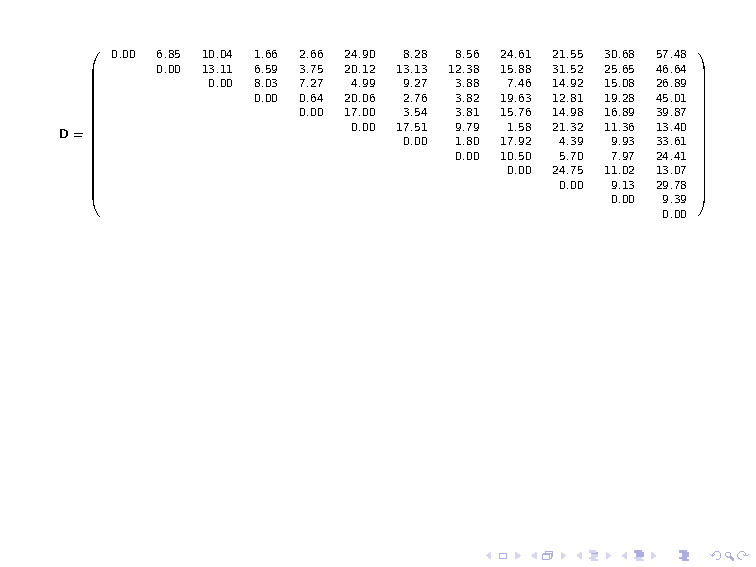
\includegraphics[scale=0.75]{dist_eucl_esc.pdf}}
\begin{center}
{\tiny
%\begin{tabular}{|@{}r@{}|@{}r@{}|@{}r@{}|@{}r@{}|@{}r@{}|@{}r@{}|@{}r@{}|@{}r@{}|@{}r@{}|@{}r@{}|@{}r@{}|@{}r@{}|}\hline
\begin{tabular}{|r@{}|r@{}|r@{}|r@{}|r@{}|r@{}|r@{}|r@{}|r@{}|r@{}|r@{}|r@{}|}\hline
0.00 &&&&&&&&&&&\\\hline                                                                                                                         
2.62&    0.00&&&&&&&&&&\\        \hline                                                                                                        
3.16&  3.62 &    0.00&&&&&&&&&\\\hline                                                                                                     
1.30 &  2.57 &  2.83 &    0.00&&&&&&&&\\        \hline                                                                                  
1.63& 1.94&  2.70&   0.80&    0.00&&&&&&&\\         \hline                                                                      
4.99&4.49&  2.23& 4.48& 4.12 &    0.00&&&&&&\\         \hline                                                           
2.88&  3.62&  3.04& 1.66&  1.88&  4.18 &   0.00&&&&&\\              \hline                                           
2.93 & 3.52& 1.97&  1.95&  1.95&  3.13&  1.34&    0.00&&&&\\     \hline                                         
4.96&3.99&  2.73& 4.43& 3.97&  1.26&  4.23&  3.24&    0.00&&&\\      \hline                             
4.64&  5.61&  3.86& 3.58&  3.87&  4.62&  2.10&  2.39&  4.99&    0.00&&\\      \hline                  
5.54&  5.07&  3.88& 4.39&  4.11& 3.37&  3.15&  2.82&  3.32&  3.02&    0.00&\\    \hline         
7.58&   6.83& 5.19& 6.71&  6.31& 3.66& 5.80&  4.94& 3.62&  5.46&  3.06 & 0.00 \\\hline  
\end{tabular}}
\end{center}}
\end{itemize}
\end{frame}
\begin{frame}
\frametitle{Caso en que la matriz $\vect{X}$ es una tabla de contingencia}
\begin{itemize}
\item<2->{$\vect{X}$ es una tabla de contingencia cuando representa una matriz de frecuencias.}
\item<3->{Definimos $x_{i\bullet}=\sum_{j=1}^p x_{ij}$ y $\frac{x_{ij}}{x_{i\bullet}}$ la distribución condicional de la fila~$i$-ésima. De la misma forma, definimos $x_{\bullet j}=\sum_{i=1}^n x_{ij}$ y $\frac{x_{ij}}{x_{\bullet j}}$ la distribución condicional de la columna $j$-ésima. Sea $x_{\bullet\bullet}=\sum_{i=1}^n  x_{i\bullet} = \sum_{j=1}^p x_{\bullet j}$.}
\item<4->{En este caso la distancia entre las filas $i_1$ e $i_2$ es la siguiente:
$$
d^2 (i_1, i_2)=\sum_{j=1}^p \frac{1}{\left(\frac{x_{\bullet j}}{x_{\bullet\bullet}}\right)} \left(\frac{x_{i_1 j}}{x_{i_1\bullet}} - \frac{x_{i_2 j}}{x_{i_2\bullet}}\right)^2.
$$}
\end{itemize}
\end{frame}
\subsection{Algoritmos jerárquicos de clúster}
\begin{frame}
\frametitle{Introducción}
\begin{itemize}
\item<2->{Existen dos métodos jerárquicos de ``clustering": algoritmos aglomerativos y algoritmos de división.}
\begin{itemize}
\item<3->{Los algoritmos  aglomerativos empiezan con la partición más fina posible (cada individuo constituye un clúster) y los va agrupando.}
\item<4->{Los algoritmos  de división empiezan con la partición más burda posible (todos los individuos constituyen el clúster) y va dividiendo los clústers en clústers más pequeños.}
\item<5->{Los algoritmos aglomerativos requieren menos tiempo de cálculo y son los más utilizados.}
\end{itemize}
\end{itemize}
\end{frame}
\iffalse
\begin{frame}
\frametitle{Introducción}
\uncover<2->{La diferencia esencial entre los dos métodos de ``clustering'' es que en los métodos jerárquicos las asignaciones de los elementos a los grupos, una vez hallados éstos, no se pueden cambiar; en cambio, en los métodos de partición, sí.}
\end{frame}
\fi
\subsubsection{Algoritmos jerárquicos. Técnicas aglomerativas.}
\begin{frame}
\frametitle{Pasos a realizar en los algoritmos aglomerativos}
\begin{itemize}
\item<2->{Construir la partición más fina posible.}
\item<3->{Calcular la matriz de distancias $D$.}
\item<4->{Realizar los pasos siguientes hasta que todos los individuos estén en un mismo clúster:}
\begin{itemize}
\item<5->{Encontrar los dos clústers con la distancia más próxima.}
\item<6->{Definir un nuevo clúster compuesto por los dos clústers anteriores encontrados.}
\item<7->{Calcular la nueva matriz de distancias reducida $D$ entre los nuevos clústers.}
\end{itemize}
\end{itemize}
\end{frame}
\begin{frame}
\frametitle{Pasos a realizar en los algoritmos aglomerativos}
\begin{itemize}
\item<2->{Si dos grupos, $P$ y $Q$ tienen que agregarse en un nuevo clúster, el cálculo de la distancia entre el nuevo clúster $P+Q$ y otro clúster cualquiera $R$ se realiza de la forma siguiente:
$$
\begin{array}{rl}
d(R,P+Q)= & \delta_1 d(R,P)+\delta_2 d(R,Q)+\delta_3 d(P,Q)+ \\ & \delta_4 |d(R,P)-d(R,Q)|,
\end{array}
$$
donde los $\delta_j$ son parámetros a escoger. Cada elección de dichos parámetros da lugar a un algoritmo aglomerativo distinto.}
\end{itemize}
\end{frame}
\begin{frame}
\frametitle{Tabla de algoritmos aglomerativos}
\uncover<2->{Definimos $n_P$ el número de objetos en el clúster $P$.
\vskip 0.25cm
\begin{tabular}{|l|@{}c|@{}c|@{}c|@{}c|}
\hline
Nombre&$\delta_1$&$\delta_2$&$\delta_3$&$\delta_4$\\\hline
Enlace simple&$1/2$&$1/2$&$0$&$-1/2$\\\hline
Enlace completo&$1/2$&$1/2$&$0$&$1/2$\\\hline
Enlace promedio&$1/2$&$1/2$&$0$&$0$\\\hline
Enlace promedio&$\frac{n_P}{n_P + n_Q}$&$\frac{n_Q}{n_P + n_Q}$&$0$&$0$\\ con pesos&&&&\\\hline
Centroide&$\frac{n_P}{n_P + n_Q}$&$\frac{n_Q}{n_P + n_Q}$&$-\frac{n_P n_Q}{(n_P + n_Q)^2}$&$0$\\\hline
Mediana&$1/2$&$1/2$&$-1/4$&$0$\\\hline
Ward&$\frac{n_R + n_P}{n_R + n_P + n_Q}$&$\frac{n_R + n_Q}{n_R + n_P + n_Q}$&$-\frac{n_R}{n_R + n_P + n_Q}$&$0$\\\hline
\end{tabular}
}
\end{frame}
\begin{frame}
\frametitle{Ejemplo}
\begin{itemize}
\item<2->{Consideremos los puntos siguientes en $\mathbb{R}^2: 
\begin{array}{l}
(5,-3),\ (2,-4),\ (-2,-1),\ (-3,0),\\ (-2,-2),\ (-2,4),\ (1,2),\ (1,4).\end{array}$
\vskip 0.05cm
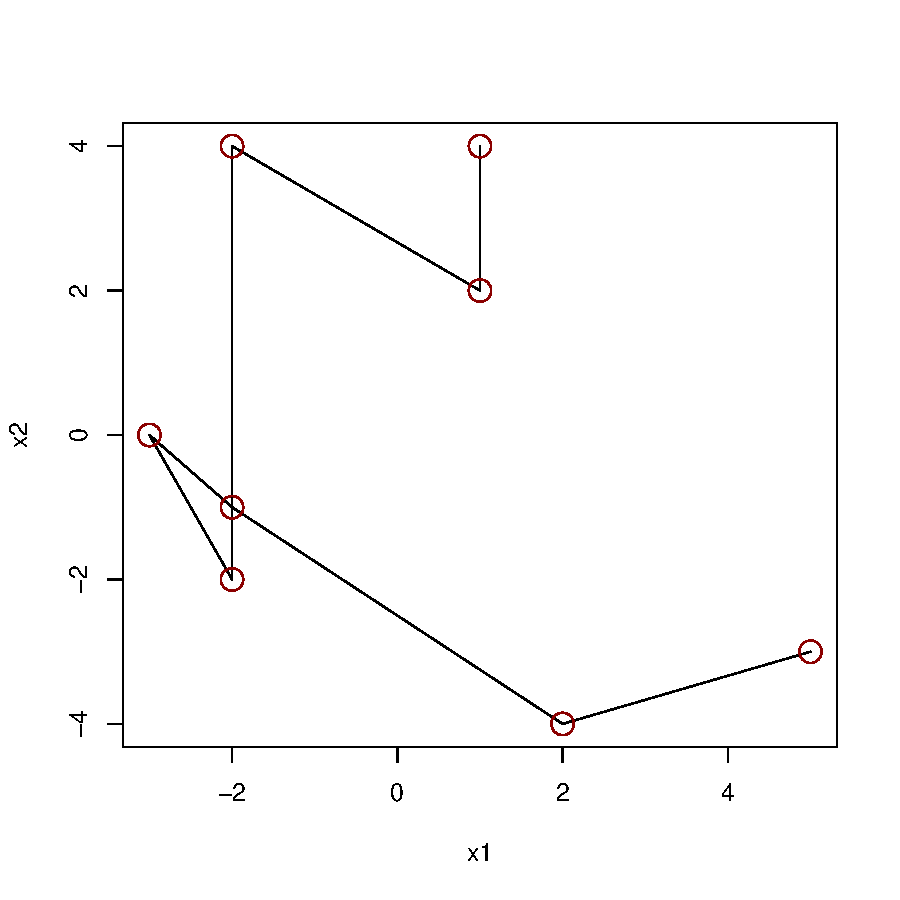
\includegraphics[scale=0.5]{ExCluster1.pdf}}
\end{itemize}
\end{frame}
\begin{frame}
\frametitle{Ejemplo}
\begin{itemize}
\item<2->{La matriz de distancias (distancia euclídea) entre los $8$ puntos es:
$$
D= \begin{pmatrix}
0.00&3.16&7.28&8.54&7.07&9.90&6.40&8.06 \\
&0.00&5.00&6.40&4.47&8.94&6.08&8.06\\
&&0.00&1.41&1.00&5.00&4.24&5.83\\
&&&0.00&2.24&4.12&4.47&5.66\\
&&&&0.00&6.00&5.00&6.71\\
&&&&&0.00&3.61&3.00\\
&&&&&&0.00&2.00\\
&&&&&&&0.00
\end{pmatrix}
$$}
\end{itemize}
\end{frame}
\begin{frame}
\frametitle{Ejemplo}
\begin{itemize}
\item<2->{Aplicación del algoritmo.
Como vemos, los puntos más cercanos son el $3$ y el $5$. Por tanto, los nuevos clústers serán:
$$
\{1\},\ \{2\},\ \{3,5\},\ \{4\},\ \{6\},\ \{7\},\ \{8\}.
$$}
\item<3->{Calculemos la nueva matriz de distancias usando el enlace simple entre los $7$ clústers:
$$
D_2 = 
\begin{pmatrix}
0.00&3.16&7.07&8.54&9.90&6.40&8.06\\
&0.00&4.47&6.40&8.94&6.08&8.06\\
&&0.00&1.41&5.00&4.24&5.83\\
&&&0.00&4.12&4.47&5.66\\
&&&&0.00&3.61&3.00\\
&&&&&0.00&2.00\\
&&&&&&0.00
\end{pmatrix}
$$}
\end{itemize}
\end{frame}
\begin{frame}
\frametitle{Ejemplo}
\begin{itemize}
\item<2->{La distancia más cercana está ahora entre los clústers $\{3,5\}$ y el clúster $\{4\}$. Los nuevos clúster son:
$$
\{1\},\ \{2\},\ \{3,4,5\},\ \{6\},\ \{7\},\ \{8\}.
$$
La nueva matriz de distancias será:
$$
D_3 =
\begin{pmatrix}
0.00&3.16&7.07&9.90&6.40&8.06\\
&0.00&4.47&8.94&6.08&8.06\\
&&0.00&4.12&4.24&5.66\\
&&&0.00&3.61&3.00\\
&&&&0.00&2.00\\
&&&&&0.00
\end{pmatrix}
$$}
\end{itemize}
\end{frame}
\begin{frame}
\frametitle{Ejemplo}
\begin{itemize}
\item<2->{La distancia más cercana se encuentra entre los clústers $\{7\}$ y $\{8\}$. Los nuevos clústers serán:
$$
\{1\},\ \{2\},\ \{3,4,5\},\ \{6\},\ \{7,8\}.
$$
La nueva matriz de distancias será:
$$
D_4 = \begin{pmatrix}
0.00&3.16&7.07&9.90&6.40\\
&0.00&4.47&8.94&6.08\\
&&0.00&4.12&4.24\\
&&&0.00&3.00\\
&&&&0.00
\end{pmatrix}
$$}
\end{itemize}
\end{frame}
\begin{frame}
\frametitle{Ejemplo}
\begin{itemize}
\item<2->{La distancia más cercana se encuentra entre los clústers $\{6\}$ y $\{7,8\}$. Los nuevos clústers serán:
$$
\{1\},\ \{2\},\ \{3,4,5\},\ \{6,7,8\}.
$$
La nueva matriz de distancias será:
$$
D_5= \begin{pmatrix}
0.00&3.16&7.07&6.40\\
&0.00&4.47&6.08\\
&&0.00&4.12\\
&&&0.00
\end{pmatrix}
$$}
\end{itemize}
\end{frame}
\begin{frame}
\frametitle{Ejemplo}
\begin{itemize}
\item<2->{La distancia más cercana se encuentra entre los clústers $\{1\}$ y $\{2\}$. Los nuevos clústers serán:
$$
\{1,2\},\ \{3,4,5\},\ \{6,7,8\}.
$$
La nueva matriz de distancias será:
$$
D_6 = \begin{pmatrix}
0.00 & 4.47 & 6.08\\
& 0.00 & 4.12\\
&&0.00
\end{pmatrix}
$$}
\end{itemize}
\end{frame}
\begin{frame}
\frametitle{Ejemplo}
\begin{itemize}
\item<2->{La distancia más cercana se encuentra entre los clústers $\{3,4,5\}$ y $\{6,7,8\}$. Los nuevos clústers serán:
$$
\{1,2\},\ \{3,4,5,6,7,8\}.
$$
La nueva matriz de distancias será:
$$
D_7 = \begin{pmatrix}
0.00 & 4.47\\
&0.00
\end{pmatrix}
$$}
\item<3->{El último paso del algoritmo será juntar los dos últimos clusters obteniendo un clúster único compuesto por los $8$ puntos.}
\end{itemize}
\end{frame}
\begin{frame}
\frametitle{Ejemplo}
\uncover<2->{Todo el ejemplo queda resumido en lo que se denomina un dendograma:
\vskip 0.05cm
%\includegraphics[scale=0.5]{DendExCluster1.pdf}}
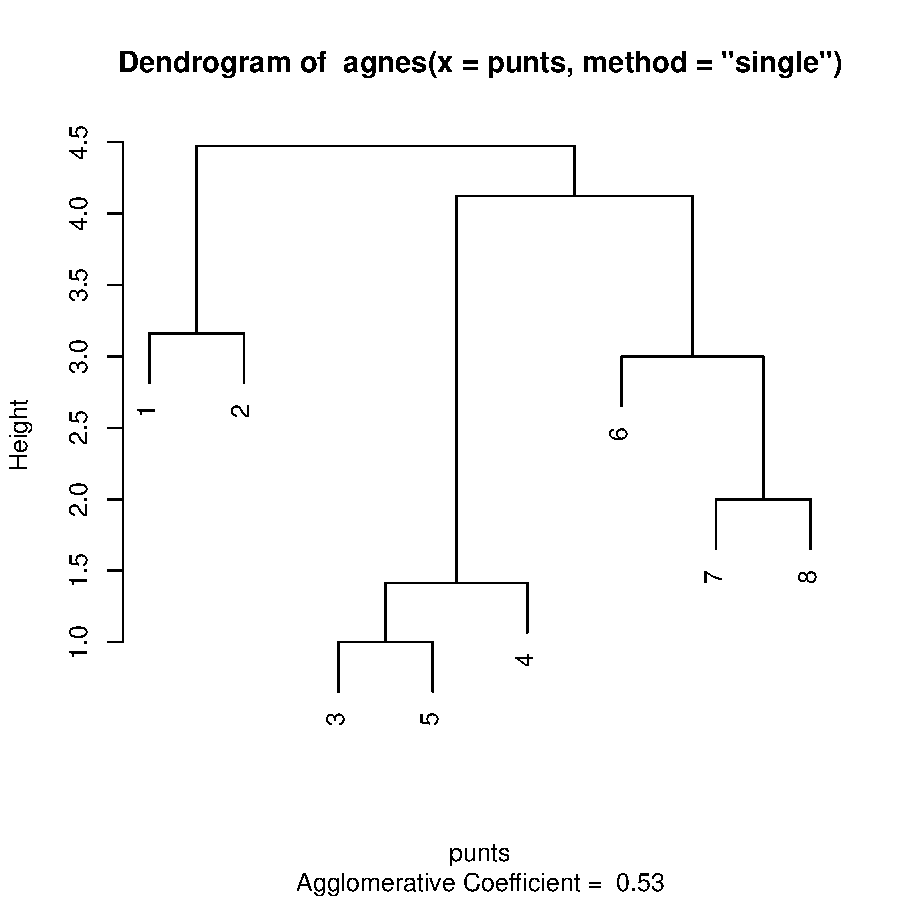
\includegraphics[scale=0.4]{DendogramaPuntsSimple.pdf}}
\end{frame}
\begin{frame}
\frametitle{Propiedades de los algoritmos aglomerativos.}
\begin{itemize}
\item<2->{En el procedimiento del enlace simple, la distancia entre el clúster $R$ y el clúster unión de $P$ y $Q$, $P+Q$ se puede hallar como:
$$
d(R,P+Q)=\min (d(R,P),d(R,Q)).
$$Por dicho motivo, se denomina algoritmo del vecino más próximo. Dicho algoritmo tiende a construir clústers grandes. Clústers que difieren pero que no están bien separados pueden unirse en un sólo clúster si tienen dos individuos próximos.} 
\end{itemize}
\end{frame}
\begin{frame}
\frametitle{Propiedades de los algoritmos aglomerativos.}
\begin{itemize}
\item<2->{En el procedimiento del enlace completo, se trata de corregir este tipo de agrupamiento considerando distancias grandes. De hecho, la distancia entre el clúster $R$ y el clúster unión de $P$ y $Q$, $P+Q$ se puede hallar como:
$$
d(R,P+Q)=\max (d(R,P),d(R,Q)).
$$Por dicho motivo, se denomina el algoritmo del vecino más alejado. Dicho algoritmo agrupa clústers donde todos los puntos están próximos.}
\item<3->{En el procedimiento del enlace promedio, se propone una solución intermedia entre los dos procedimientos anteriores. En este caso, se calcula la distancia promedio:
$$
d(R,P+Q)=\frac{n_P}{n_P + n_Q} d(R,P)+\frac{n_Q}{n_P + n_Q} d(R,Q).
$$}
\end{itemize}
\end{frame}
\begin{frame}
\frametitle{Propiedades de los algoritmos aglomerativos.}
\begin{itemize}
\item<2->{El procedimiento del centroide es similar al procedimiento promedio pero usa la distancia geométrica entre el clúster $R$ y el centro de gravedad promediado entre los clústers $P$ y $Q$.}
\item<3->{El algoritmo de Ward se diferencia de los otros procedimientos respecto de la unificación. Dicho algoritmo no junta grupos con distancias pequeñas sino que junta grupos en los que no se incremente la heterogeneidad de los mismos ``demasiado". El objetivo de dicho procedimiento es que la variación dentro de los clústers no aumente de forma drástica. El resultado es que los grupos son lo más homogéneos posible.}
\end{itemize}
\end{frame}
\begin{frame}
\frametitle{Ejemplo}
\uncover<2->{El dendograma usando el método completo para el ejemplo anterior es:
\vskip 0.05cm
%\includegraphics[scale=0.5]{DendExCluster1.pdf}}
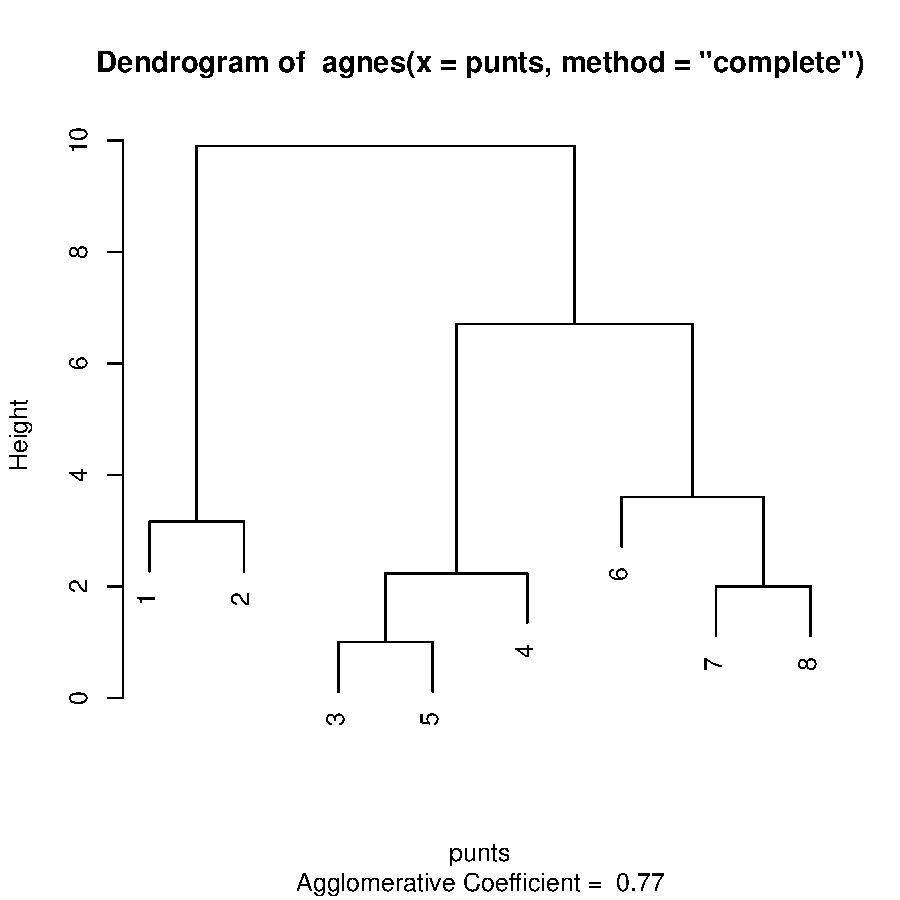
\includegraphics[scale=0.4]{DendogramaPuntsComplet.pdf}}
\end{frame}
\begin{frame}
\frametitle{Ejemplo}
\uncover<2->{El dendograma usando el método promedio para el ejemplo anterior es:
\vskip 0.05cm
%\includegraphics[scale=0.5]{DendExCluster1.pdf}}
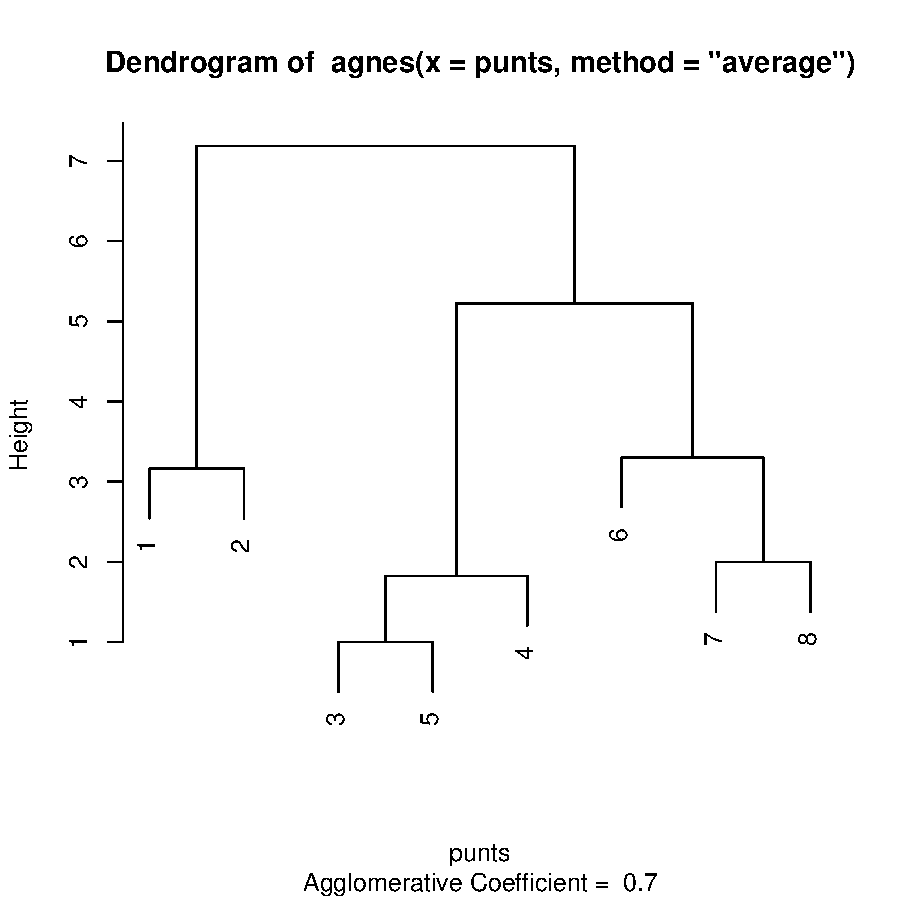
\includegraphics[scale=0.4]{DendogramaPuntsAverage.pdf}}
\end{frame}
\begin{frame}
\frametitle{Ejemplo}
\uncover<2->{El dendograma usando el método de Ward para el ejemplo anterior es:
\vskip 0.05cm
%\includegraphics[scale=0.5]{DendExCluster1.pdf}}
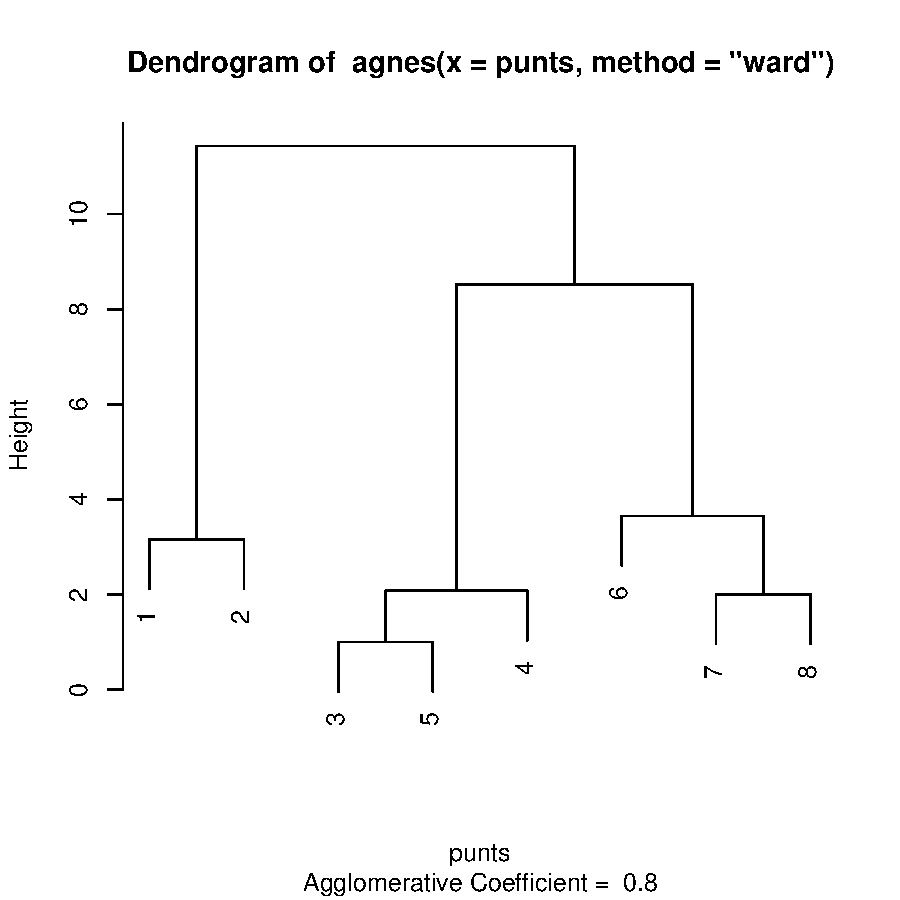
\includegraphics[scale=0.4]{DendogramaPuntsWard.pdf}}
\end{frame}
\begin{frame}
\frametitle{Propiedades de los algoritmos aglomerativos.}
\begin{itemize}
\item<2->{Se define la heterogeneidad de un clúster $R$ como:
$$
I_R = \frac{1}{n_R} \sum_{i=1}^{n_R} d^2(x_i,\overline{x}_R),
$$
donde $\overline{x}_R$ es el centro de gravedad o la media del clúster $R$. Si $d$ es la distancia euclídea, $I_R$ representa la varianza del clúster $R$.}
\item<3->{Cuando dos clústers $P$ y $Q$ se unen, el nuevo clúster $P+Q$ tiene una heterogeneidad $I_{P+Q}$. Puede demostrarse que el aumento de heterogeneidad viene dada por:
$$
\Delta (P,Q)= \frac{n_P n_Q}{n_P + n_Q} d^2 (P,Q).
$$}
\item<4->{El algoritmo de Ward, por tanto, puede definirse como el algoritmo que minimiza $\Delta (P,Q)$.}
\end{itemize}
\end{frame}
